\documentclass[tikz,border=10pt]{standalone}
\usepackage{tkz-euclide}
\usetikzlibrary{intersections, calc, angles, quotes}

\begin{document}
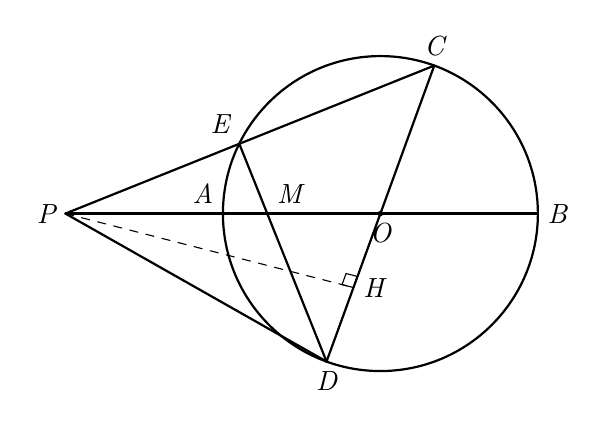
\begin{tikzpicture}[line join=round, line cap=round, >=stealth, font=\itshape]
    % 1. 定义基本参数
    \pgfmathsetmacro{\r}{2}      % 圆的半径
    \coordinate (O) at (0,0);    % 圆心 O
    
    % 2. 绘制圆
    \draw[thick] (O) circle (\r);
    \fill (O) circle (1pt); % 标记圆心点
    
    % 3. 定义点 B, A (水平直径)
    \coordinate (B) at (0:\r);
    \coordinate (A) at (180:\r);
    \draw[thick] (A) -- (B);
    
    % 4. 定义点 C, D (倾斜直径)
    % 设定 C 点角度大约为 110 度
    \coordinate (C) at (70:\r);
    \coordinate (D) at ($(O)!-1!(C)$); % D 是 C 关于 O 的对称点
    \draw[thick] (C) -- (D);
    
    % 5. 绘制切线和延长线
    % 计算 C 点的切线方向：切线垂直于半径 OC
    % 设定 P 点在水平线 OA 的延长线上
    % 为了符合原图视觉效果，我们手动寻找切线与水平线的交点 P
    \coordinate (P) at (-4, 0); 
    \draw[thick] (P) -- (C);
    \draw[thick] (P) -- (A); % 延长线连接到 P
    \draw[thick] (P) -- (D);
    
    % 6. 计算交点 E
    % E 是切线 PC 与圆的另一个交点？ 
    % 观察原图：E 位于圆周上，且在线段 PC 上。
    % 这里通常有两种理解：1.PC是切线（C为切点）；2.PE是切线（E为切点）。
    % 根据图形视觉，C更像是切点，E是直线与圆的另一个交点。
    \path [name path=circle] (O) circle (\r);
    \path [name path=linePC] (P) -- (C);
    \path [name intersections={of=circle and linePC, by={E}}];
     \draw[thick] (E) -- (D);

       \path [name path=linePO] (P) -- (O);
         \path [name path=lineED] (E) -- (D);
          \path [name intersections={of=lineED and linePO, by={M}}];

   
    \coordinate (H) at ($(D)!0.25!(C)$);
    \draw[dashed] (P) -- (H);
    \tkzMarkRightAngle[size=0.15](P,H,C)
    
    % 7. 标注字母标签
    % 使用 pos 和 xshift/yshift 微调位置避开线条
    \node[below] at (O) {O};
    \node[right] at (B) {B};
    \node[above left] at (A) {A};
    \node[above] at (C) {C};
     \node[above right] at (M) {M};
    \node[below] at (D) {D};
    \node[left] at (P) {P};
     \node[right] at (H) {H};
    \node[above left] at (E) {E};

\end{tikzpicture}
\end{document}